\begin{frame}
	\frametitle{Das Erdsystem - Zusammenfassung}
	\begin{columns}
		\column{0.3\linewidth}
			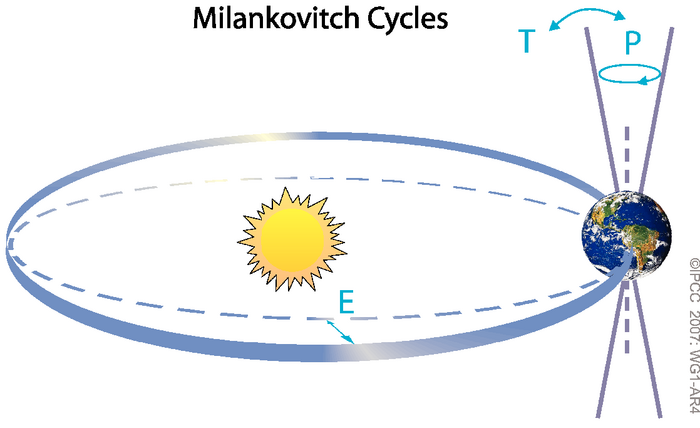
\includegraphics[width=0.9\linewidth]{bilder/milankovitch_IPCC2007_AR4.png}
		\column{0.7\linewidth}
			\begin{itemize}
				\item Das (durchschnittliche) Wetter macht das Klima, das Klima bestimmt das (wahrscheinliche) Wetter.
				\item Ursachen für natürliche Klimaänderungen: Neigung der Erdachse (Jahreszeiten) und Milankovitch Zyklen (Eiszeitzyken).
			\end{itemize}
	\end{columns}
	\begin{columns}
		\column{0.7\linewidth}
			\begin{itemize}
				\item Atmosphäre und Strahlungshaushalt der Erde erzeugen lebensfreundliche Bedingungen auf der Erde
				\item Der natürliche Treibhauseffekt entsteht vorallem durch Wasserdampf und CO$_2$.
			\end{itemize}
		\column{0.3\linewidth}
			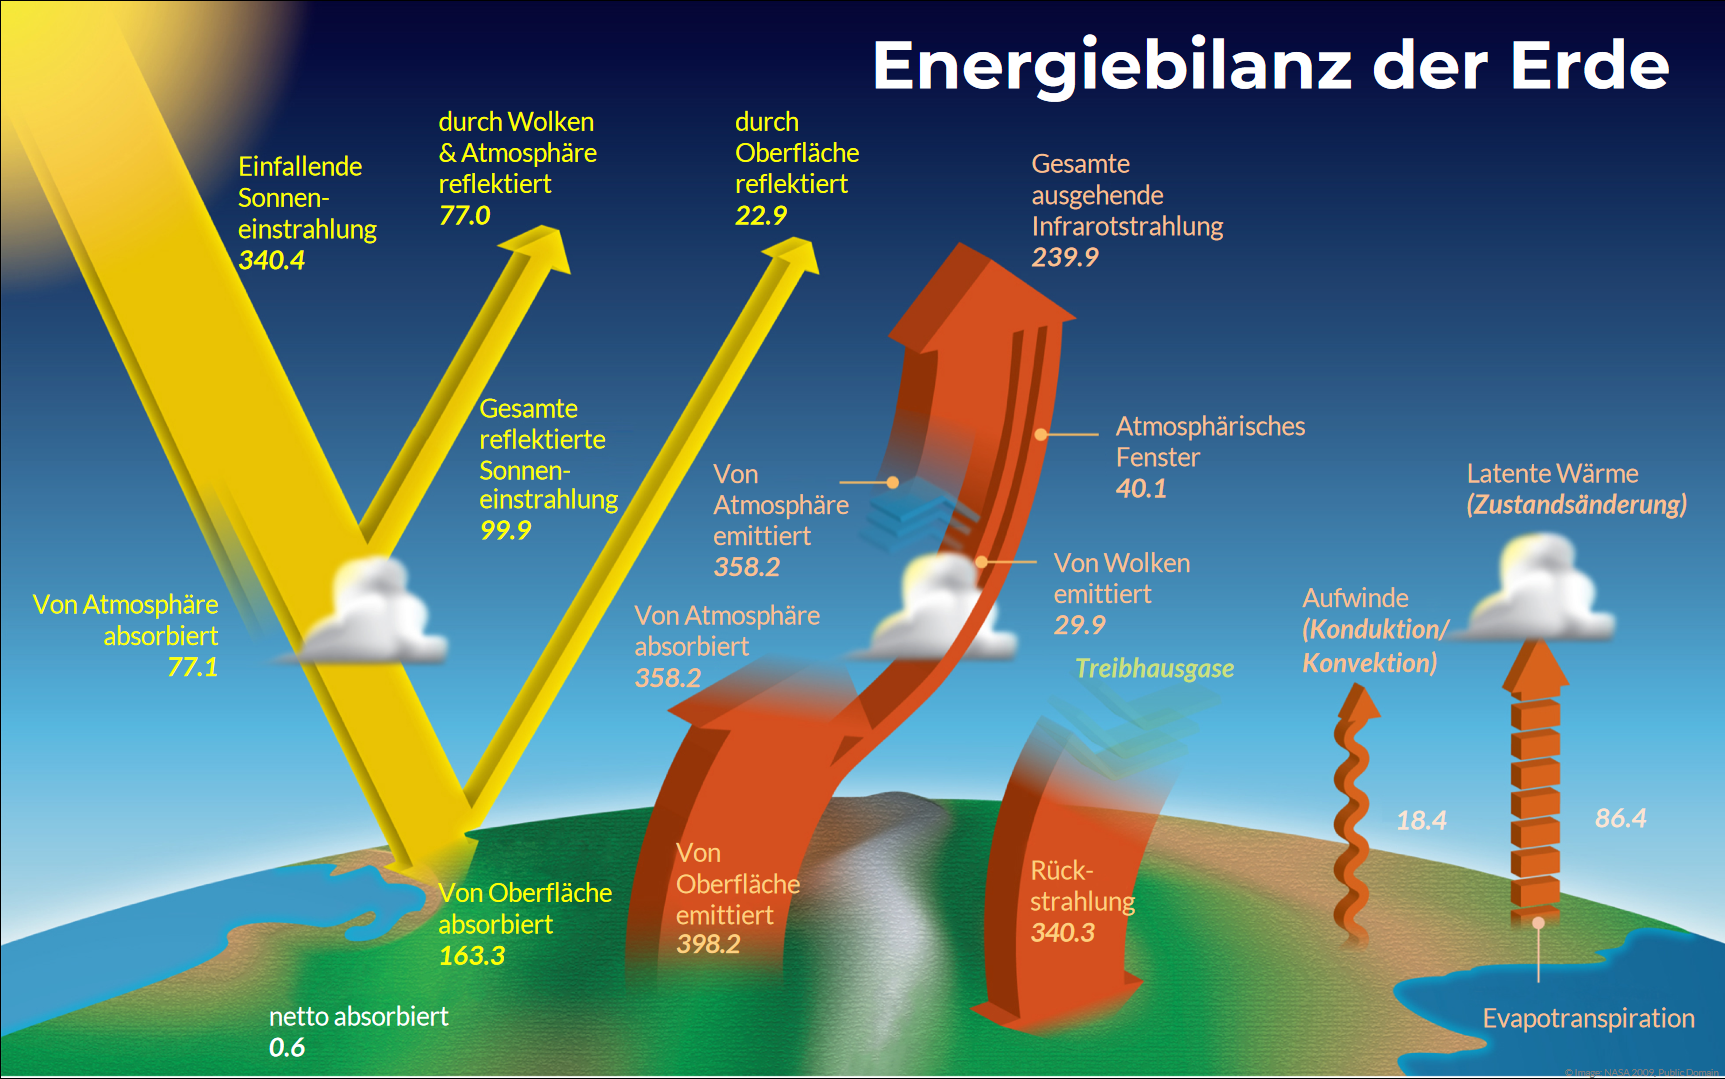
\includegraphics[width=0.9\linewidth]{bilder/Energiebilanz_der_Erde_NASA.png}
	\end{columns}
	\begin{columns}
		\column{0.3\linewidth}
			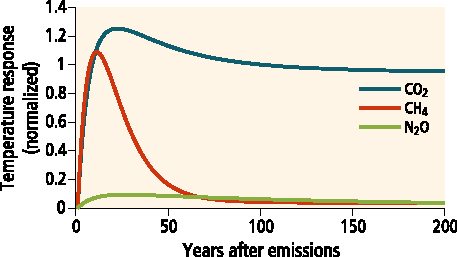
\includegraphics[width=0.9\linewidth]{bilder/ghg-forcings-over-time.pdf}
		\column{0.7\linewidth}
			\begin{itemize}
				\item CO$_2$, CH$_4$ und N$_2$O sind starke Treibhausgase, die lange in der Atmosphäre verbleiben
				\item Durch den Anstieg der atmosphärischen Konzentrationen dieser Gase seit der Industrialisierung kann der Mensch als Ursache angenommen werden.
			\end{itemize}
	\end{columns}
\end{frame}
